Veamos como se comporta el fenómeno de Gibbs en la siguiente función:
\begin{align*}
  h(t)= 
  \begin{cases}
    \frac{1}{2}-t, &\text{ cuando } 0<t\leq \frac{1}{2} \text{,} \\
    0, &\text{ cuando } t=0,\\
    -\frac{1}{2}-t, &\text{ cuando }-\frac{1}{2}\leq t<0.
  \end{cases}
\end{align*}
\begin{figure}[H]
\begin{center}
  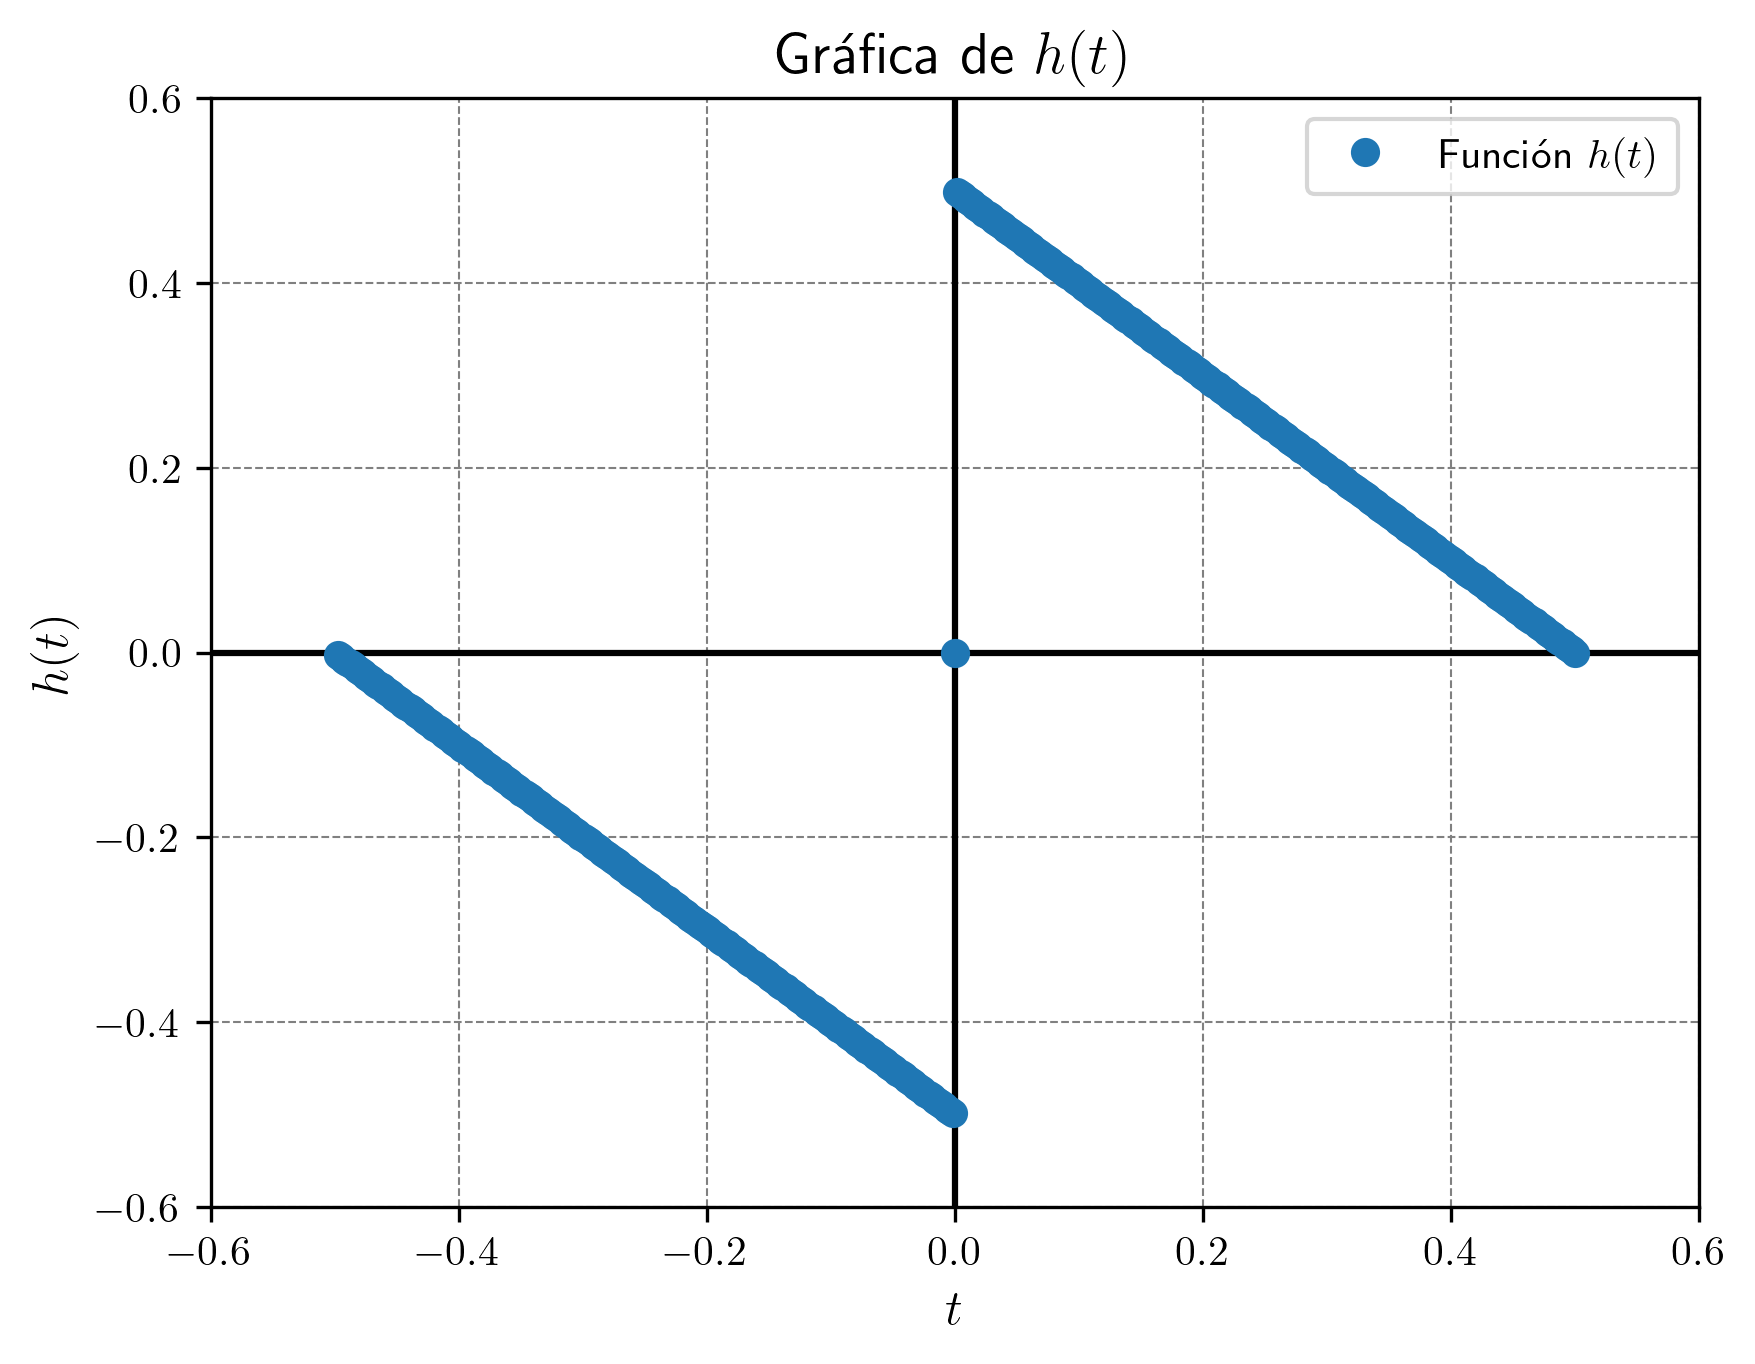
\includegraphics[scale=0.5]{Figures/h.png}
\end{center}
\end{figure}
Luego, es claro que $h$ es de variación acotada y continua excepto en el punto $t=0$, en dónde tiene una discontinuidad de salto. Además, note que $h$ es una función impar, por lo que podemos cálcular su transformada de Fourier de la siguiente manera:
\begin{equation}\label{eq:h_transformada}
  \begin{split}
    \hat{h}(m)&=\int_{\frac{-1}{2}}^{\frac{1}{2}}h(t)e^{-2\pi itm}dt,\\
    &=-2i \int_{0}^{\frac{1}{2}}\left( \frac{1}{2}-t \right)\sen(2\pi mt)dt,\\
    &=-\frac{i}{2m\pi}.  
  \end{split}
\end{equation}
Cuando $m\neq 0$ y por otro lado $\hat{h}(0)=0$.\\
Luego, las sumas parciales de Fourier de $h$ son:
\begin{equation}\label{eq:serie_h}
  \begin{split}    
    (h*D_{N})(t)&=-\frac{i}{2\pi}\sum_{\substack{|m| \leq N \\ m \neq 0}}\frac{e^{2\pi i mt}}{m}.
  \end{split}
\end{equation}
Ahora derivando respecto a $t$
\begin{equation}\label{eq:derivada_h}
  \begin{split}
    \frac{d}{dt}(h*D_{N})&=\sum_{\substack{|m| \leq N \\ m \neq 0}}e^{2\pi imt},\\
    &=D_{N}(t)-1.    
  \end{split}
\end{equation}
Siendo así, definamos $g(s)=\frac{1}{\sen(\pi s)}-\frac{1}{\pi s}$, luego utilizando el teorema fundamental del cálculo en $\ref{eq:derivada_h}$ podemos afirmar que
\begin{equation}\label{eq:convolucion}
  \begin{split}
    (h*D_{N})(t)&=\int_{0}^{t}D_{N}(s)-1ds\\
    &=-t + \int_{0}^{t}D_{N}(s)ds\\
    &=-t + \int_{0}^{t}\frac{\sen((2N+1)\pi s)}{\sen(\pi s)}ds\\
    &=-t + \int_{0}^{t}\frac{\sen((2N+1)\pi s)}{\sen(\pi s)}-\frac{\sen((2N+1)\pi s)}{\pi s}+\frac{\sen((2N+1)\pi s)}{\pi s}ds\\
    &=-t + \int_{0}^{t}g(s)\sen((2N+1)\pi s)ds +\int_{0}^{t}\frac{\sen((2N+1)\pi s)}{\pi s}ds.
  \end{split}
\end{equation}
Además, se puede ver que
\begin{align*}
  \lim_{s \to 0}g(s)&=\lim_{s \to 0}\frac{1}{\sen(\pi s)}-\frac{1}{\pi s},\\
  &=\lim_{s \to 0}\frac{\pi s-\sen(\pi s)}{\sen(\pi s)\pi s},\\
  &=\lim_{u \to 0}\frac{u-\sen(u)}{\sen(u)u},\\
  &=\lim_{u \to 0}\frac{1-\cos(u)}{\cos(u)u+\sen(u)},\\
  &=\lim_{u \to 0}\frac{\sen(u)}{-\sen(u)u+2\cos(u)},\\
  &=\frac{0}{2},\\
  &=0.
\end{align*}
Por lo que podemos asegurar que $g$ es continua en $0$ y además $g(0)=0$, luego
\begin{align*}
  \lim_{s \to 0}\frac{g(s)}{s}&=\pi\lim_{u \to 0}\frac{u-\sen(u)}{\sen(u)u^2},\\
  &=\pi \lim_{u \to 0}\frac{1-\cos(u)}{\cos(u)u^2+2\sen(u)u},\\
  &=\pi \lim_{u \to 0}\frac{\sin(u)}{-\sen(u)u^2+4\cos(u)u+2\sen(u)},\\
  &=\pi \lim_{u \to 0}\frac{\cos(u)}{-\cos(u)u^2-6\sen(u)u+6\cos(u)},\\
  &=\frac{\pi}{6}.
\end{align*}
De esto que $g(s)$ sea continua y diferenciable en $[0,\frac{1}{2}]$ y $g'(0)=\frac{\pi}{6}$, además es claro que $g$ y $g'$ son funciones no negativas crecientes en el intervalo $[0,\frac{1}{2}]$, luego
\begin{align*}
  g'(s)&=\left( \frac{1}{\sen(\pi s)}-\frac{1}{\pi s} \right)',\\
  &=-\frac{\pi\cos(\pi s)}{\sen^2(\pi s)}+\frac{1}{\pi s^2},\\
  &\leq -\frac{\pi\cos(\pi/2)}{\sen^2(\pi/2)}+\frac{4}{\pi},\\
  &\leq \frac{4}{\pi}.
\end{align*}
Ahora, utilizando esto se sigue que
\begin{equation}\label{eq:O-grande-h}
  \begin{split}
    \left|\int_{0}^{t}g(s)\sen((2N+1)\pi s)ds\right|&=\left|-\frac{\cos((2N+1)\pi t)}{(2N+1)\pi}g(t)+\int_{0}^{t}g'(s)\frac{\cos((2N+1)\pi s)}{(2N+1)\pi}ds\right|,\\
    &\leq \left( \frac{g(\frac{1}{2})}{\pi}+\frac{1}{2}\frac{g'(\frac{1}{2})}{\pi} \right)\frac{1}{2N+1},\\
    &\leq O\left( \frac{1}{2N+1} \right).
  \end{split}
\end{equation}
Luego, reemplazando $\ref{eq:O-grande-h}$ en $\ref{eq:convolucion}$ nos queda que
\begin{equation}\label{eq:6}
  \begin{split}
    (h*D_{N})(t)&=-t+\frac{1}{\pi}\int_{0}^{t}  \frac{\sen((2N+1)\pi s)}{s}ds+O\left( \frac{1}{2N+1} \right),\\
    &=-t+\frac{1}{\pi}\int_{0}^{(2N+1)\pi t}  \frac{\sen((s)}{s}ds+O\left( \frac{1}{2N+1} \right),\\
  \end{split}
\end{equation}
Ahora note que si tomamos $t\in(0,\frac{1}{2}]$, entonces $\lim_{N \to infty}(h*D_N)(t))=-t+\frac{1}{\pi}\frac{\pi}{2}=\frac{1}{2}-t$, lo que se espera del núcleo de Dirichlet. De igual forma si tomamos $t\in[-\frac{1}{2},0)$, entonces $\lim_{N \to \infty}(h*D_N)(t)=-t-\frac{1}{\pi}\frac{\pi}{2}=-\frac{1}{2}-t$. También note que para $t=0$ se cumple que $\lim_{N \to \infty}(h*D_{N})(0)=0$, por lo que podemos ver que la serie de $h$ converge al promedio de $h(0+)$ y $h(0-)$, que resulta ser $h(0)=0$.\\
Con la intención de estimar la no uniformidad de la convergencia haremos lo siguiente
\begin{align*}
  (h*D_N)(t)-\left( \frac{1}{2}-t \right)&=\frac{1}{\pi}\int_{0}^{(2N+1)\pi t}\frac{\sen(s)}{s}ds-\frac{1}{2}+O\left( \frac{1}{2N+1} \right).
\end{align*}
luego si tomamos $N=1,2,\cdots$ y $t\in (0,\frac{1}{2}]$ se cumple que
\begin{align*}
  (h*D_N)(t)-h(t)&\leq \frac{Si((2N+1)\pi)}{\pi}-\frac{1}{2}+\frac{1}{\pi}\frac{1}{2N+1},\\
  &\leq \frac{Si(\pi)}{\pi}-\frac{1}{2}+\frac{1}{\pi}\frac{1}{2N+1},\\
  &\leq 0.08949\cdots+\frac{\pi^{-1}}{2N+1}.
\end{align*}
Luego escogiendo una subsucesión $t_N\to 0$ nosotros tenemos que
\begin{equation}\label{eq:cota}
  \limsup_{N\to\infty}\left[ (h*D_{N})(t_{N})-h(t_{N}) \right]\leq \frac{Si(\pi)}{\pi}-\frac{1}{2}=0.08949\cdots,
\end{equation}
Luego, es particular si tomamos $t_N=\frac{1}{2N+1}$ se cumple que
\begin{align*}
  \limsup_{N\to\infty}\left[ (h*D_{N})(t_N)-h(t_{N}) \right]=\frac{Si(\pi)}{\pi}-\frac{1}{2}=0.08949\cdots
\end{align*}
Veamos esto gráficamente
\begin{figure}[H]
\begin{center}
  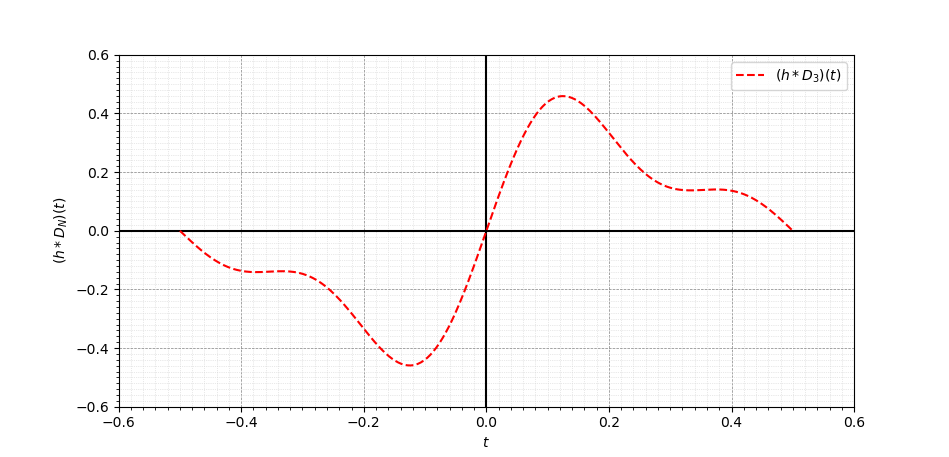
\includegraphics[scale=0.31]{Figures/3-serie.png}
  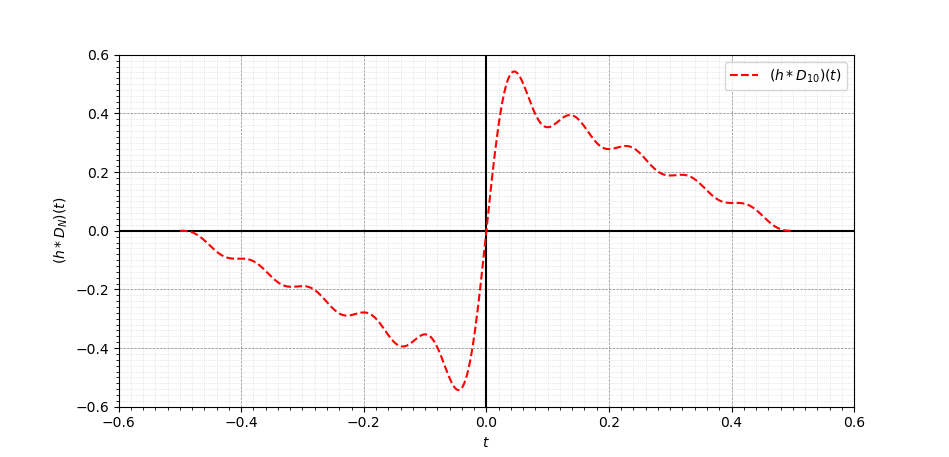
\includegraphics[scale=0.31]{Figures/10-serie.png}\\
  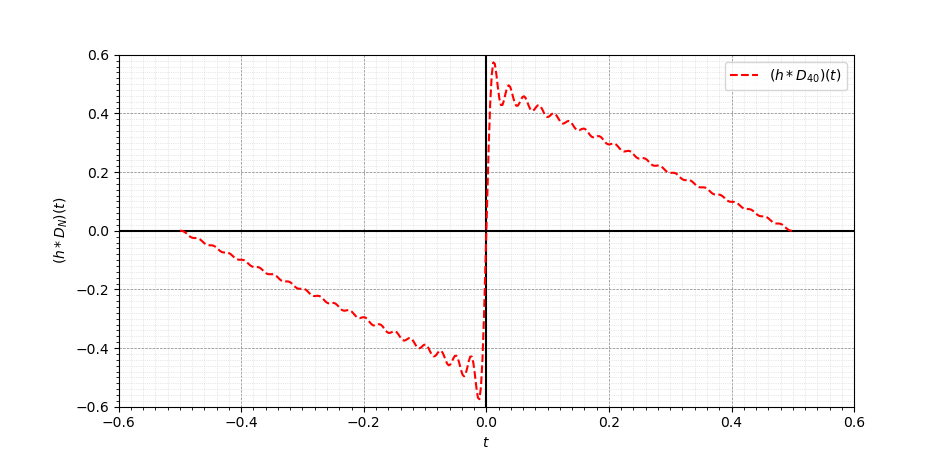
\includegraphics[scale=0.31]{Figures/40-serie.png}
  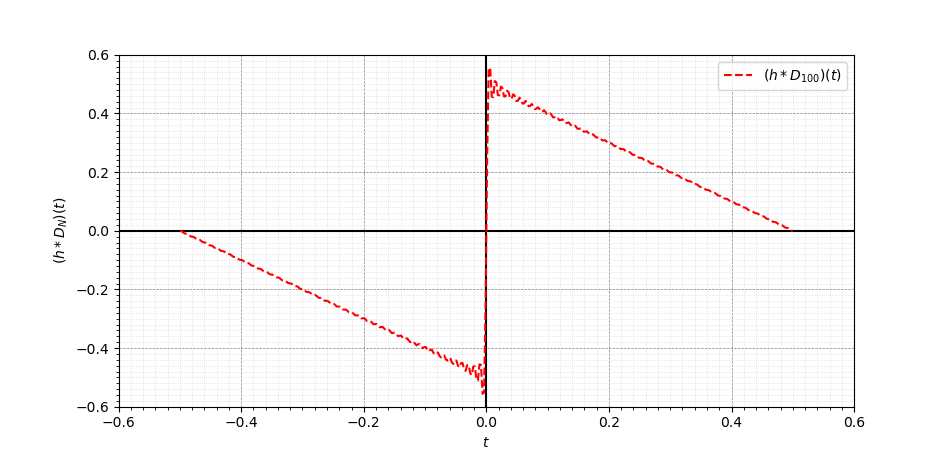
\includegraphics[scale=0.31]{Figures/100-serie.png}
\end{center}
  \caption{Series de Fourier $N=3,10,40$ y $100$.}
\label{fig:series-de-fourier-h}
\end{figure}
En dónde se puede ver que las series presentan superar en un $9\%$ aproximadamente al acercarse al salto del $0$, a este suceso se le llama el fenómeno de Gibbs. 

